%==============================================================
%  [한글판] 어떤 데이터가 어떤 분류기에 맞는가?
%
%  ※ Overleaf 컴파일러를 반드시 XeLaTeX 로 설정하세요 (한글: kotex).
%    Menu -> Compiler -> XeLaTeX.   pdfLaTeX는 한글이 안 됩니다.
%    참고문헌: xelatex -> bibtex -> xelatex x2
%  업로드 파일: main_kr.tex, refs.bib, fig_augmentation.pdf
%==============================================================
\documentclass[conference]{IEEEtran}

\usepackage{kotex}            % 한글 (XeLaTeX)
\usepackage{amsmath,amssymb}
\usepackage{booktabs}
\usepackage{array}
\usepackage{graphicx}
\usepackage{tikz}
\usetikzlibrary{shapes.multipart, positioning, arrows.meta, calc}
\usepackage{listings}
\usepackage{xcolor}
\usepackage{url}
\usepackage{hyperref}

\lstset{
  basicstyle=\ttfamily\footnotesize,
  keywordstyle=\color{blue!70!black}\bfseries,
  commentstyle=\color{green!40!black}\itshape,
  stringstyle=\color{red!60!black},
  numbers=none, breaklines=true, showstringspaces=false,
  language=Python, frame=single, framesep=3pt,
  aboveskip=14pt,
  belowskip=8pt,
}
% listings 캡션이 코드 프레임과 겹치지 않도록 간격 확보
\setlength{\abovecaptionskip}{4pt}
\setlength{\belowcaptionskip}{7pt}

\begin{document}

\title{어떤 데이터가 어떤 분류기에 맞는가? 한국어 NLI에서 모델별·도메인별
데이터 적합성을 위한 객체지향 테스트베드}

\author{
\IEEEauthorblockN{이다원 (Dawon Lee)}
\IEEEauthorblockA{건국대학교 컴퓨터공학부\\
서울, 대한민국\\
rudaa1018@gmail.com}
}

\maketitle

%--------------------------------------------------------------
\begin{abstract}
머신러닝 실무의 흔한 직관은, 분류기마다 그리고 데이터 도메인마다 서로
다른 학습 데이터가 필요하다는 것이다. 본 연구는 이 직관을 한국어 자연어
추론(NLI) 위에서 통제된 객체지향 실험으로 바꾼다. 세 분류기---$k$-최근접
이웃(KNN), NumPy로 직접 구현한 신경망(NN), 파인튜닝 BERT---를 하나의
\texttt{Classifier} 추상 아래 치환 가능하게 구현하고, 짝을 이루는
\texttt{Domain}/\texttt{TrainingStrategy} 추상으로 KLUE-NLI를 목표 도메인과
학습 전략의 곱으로 만든다. 모델 효과로는 BERT가 임베딩 기반 분류기를 크게
앞선다. 핵심 질문---목표 도메인에서 잘하려면 그 도메인만 학습(targeted)
할까, 전체 풀을 학습(broad)할까---은 작은 in-domain 베이스라인을 targeted
또는 broad 데이터로 증강해 답한다: 잘 대표된 목표에선 구성이 무의미하지만,
과소대표된 목표에선 in-domain 증강이 예제당 더 효율적이나 희소 풀에 의해 상한이
정해지며, 그 너머 broad 증강의 이득은 모델 용량에 비례한다(천장 너머 BERT $+0.037$
macro-F1, KNN·NN $\approx +0.004$). 한편 정확도와 매크로F1의 격차는 정확도만으로는
가려지는 동작 차이를 드러낸다---NN은 가장 쉬운 클래스로 붕괴해 정확도를
부풀린다. 모든 결과는 이 데이터 한정으로 보고하며, 일반적 우월성은
주장하지 않는다.
\end{abstract}

\begin{IEEEkeywords}
객체지향 설계, 자연어 추론, 한국어 NLP, $k$-최근접 이웃, 신경망, BERT,
데이터 적합성
\end{IEEEkeywords}

%--------------------------------------------------------------
\section{서론}
\label{sec:intro}
실무자들은 흔히 ``올바른'' 학습 데이터가 \emph{무엇을} 학습시키는가에 달려
있다고 가정한다---최근접 이웃, 작은 신경망, 대형 사전학습 트랜스포머가 각기
다른 데이터에서 이득을 본다고, 한 모델도 도메인에 따라 다르게 동작한다고.
이런 가정은 보통 비격식적으로만 언급된다. 본 논문은 이를 통제된 실험의
대상으로 삼아, 객체지향(OO) 설계를 그 비교가 공정하도록 유지하는 도구로
사용한다. 이 주제는 저자가 지향하는 데이터 중심 한국어 NLP와 맞닿아
있다---거기서는 \emph{주어진 모델에 어떤 데이터가 맞는가}가 반복되는 실무적
물음이며, 비교를 깔끔한 OO 시스템으로 구축하는 것은 과목 과제이자 그 연구
관심으로 가는 작은 걸음이다.

대상은 한국어 NLI다---전제와 가설이 주어질 때, 가설이 전제에 대해
\emph{함의}·\emph{중립}·\emph{모순} 중 무엇인지 판정한다. 공개 벤치마크
KLUE-NLI~\cite{park2021klue}는 각 예제에 \emph{출처}를 표기해 원칙적인 도메인
분할을 가능하게 한다.

기여는 둘이다.
\begin{itemize}
  \item \textbf{(G1) 치환 가능한 분류기 계층.} KNN, 직접 구현 NumPy 신경망,
        파인튜닝 BERT를 하나의 추상 \texttt{Classifier} 아래 구현. 같은 계약을
        만족(리스코프 치환 원칙)하고, 새 분류기는 실험 루프를 건드리지 않고
        서브클래스로 추가(개방--폐쇄 원칙).
  \item \textbf{(G2) 목표\,$\times$\,전략 설계, 목표별 평가.}
        \texttt{Domain}/\texttt{TrainingStrategy} 추상으로, 목표 도메인만
        학습(\emph{targeted}) vs 전체 학습(\emph{broad})이 그 도메인에서 나은지
        를 목표의 test 슬라이스에서 동일 데이터량으로 비교. 전체셋 평가가 부르는
        test-구성 아티팩트를 회피.
\end{itemize}
이와 더불어 전 구간에서 정확도가 아니라 매크로F1을 보고하는데, 이는 정확도만으로는
가려지는 모델별 동작(NN의 클래스 붕괴)을 드러낸다. 다만 이는 위 두 기여를 뒷받침하는
\emph{방법론적 선택}으로 다루며 별도의 기여로 세우지 않는다(\ref{sec:pertarget}절).

\paragraph*{범위와 입장}
모든 정량 결과는 이 데이터·예산 한정으로 성립하며, 어떤 모델이 일반적으로
낫다고 주장하지 않는다. 세 분류기는 \emph{유비}로서 생성형 시스템의 이질적
구성요소의 대리물 역할을 할 뿐, 동일하다고 주장하지 않는다(유비일 뿐 동일성
아님). 유일한 진짜 기술적 다리는 BERT 계열 문장 임베딩이 우리 KNN/NN 특징
공간과 현대 의미 매칭 파이프라인 양쪽의 바탕이라는 점이다(\ref{sec:conclusion}절).

%--------------------------------------------------------------
\section{관련 연구}
\label{sec:related}
\paragraph*{객체지향 설계}
클래스 구조는 GoF의 전략 패턴~\cite{gamma1994design}과, 구체적으로 Lott \&
Phillips의 최근접 이웃 사례~\cite{lott2021python}(\texttt{Sample}/
\texttt{TrainingData}/\texttt{Hyperparameter} 분해)를 문장쌍에 맞게 변형하고
단일 거리 규칙에서 추상 \texttt{Classifier} 계열로 일반화한다.

\paragraph*{분류기}
서로 다른 시대·귀납편향에서 선택했다---사례 기반 최근접 이웃
\cite{cover1967nearest}, 오차 역전파 신경망~\cite{rumelhart1986learning}(순/
역전파를 드러내려 NumPy로 재구현), 종단간 파인튜닝 BERT~\cite{devlin2019bert}.
임베딩 기반 모델은 Sentence-BERT~\cite{reimers2019sentence}로 인코딩한다.
평가 관행은 scikit-learn 생태계~\cite{pedregosa2011scikit}를 따르되, 지표와
신경망은 직접 구현했다.

\paragraph*{한국어 NLI}
KLUE-NLI~\cite{park2021klue}. 예제별 출처 표기로 통제된 도메인 분할이 가능하다.

%--------------------------------------------------------------
\section{제안하는 객체지향 시스템}
\label{sec:system}

\subsection{두 축: 모델과 데이터}
모델 축(KNN, NN, BERT)과 데이터 축. 먼저 단순 학습 분할(격식체 vs 통합)을
전체 평가셋으로 읽어 함정---혼합 test셋으로 데이터 선택을 비교하면 목표가
test 구성과 뒤섞임---을 드러낸 뒤(\ref{sec:results}절),
\texttt{Domain}/\texttt{TrainingStrategy} 추상으로 데이터 축을 제대로 다뤄
\emph{목표별} targeted와 broad를 비교한다(\ref{sec:pertarget}절). 두 불변식이
비교를 해석 가능하게 한다: 모든 학습 풀은 라벨 균형 표본, 평가셋은 고정(목표별
슬라이스).

\subsection{클래스 구조}
그림~\ref{fig:uml}이 계층을 보인다. 데이터는 캡슐화된 \texttt{NLISample}(두
문장)과 라벨 붙은 \texttt{KnownNLI}로, 둘 다 \texttt{from\_dict} 팩토리로
생성되어 잘못된 입력에 커스텀 \texttt{InvalidSampleError}(\texttt{ValueError}
서브클래스, \texttt{raise\ldots from})를 던진다. 표현은 추상 \texttt{Embedder},
의미는 추상 \texttt{Classifier}가 담당한다.

\begin{figure*}[t]
\centering
\begin{tikzpicture}[
  umlclass/.style={draw, rectangle split, rectangle split parts=2,
    fill=blue!4, text width=2.5cm, align=left, font=\ttfamily\scriptsize, inner sep=3pt},
  abstractclass/.style={umlclass, fill=orange!10},
  inh/.style={-{Triangle[open, length=3mm, width=3mm]}, thick},
  use/.style={-{Stealth[length=2mm]}, dashed, gray!70!black},
  note/.style={font=\itshape\scriptsize, text width=3cm, align=center}]
\node[umlclass] (sample) at (0,0)
  {\textbf{NLISample}\nodepart{second}+premise\\+hypothesis\\+from\_dict()};
\node[abstractclass] (emb) at (4.7,0)
  {\textbf{$\langle\langle$abstract$\rangle\rangle$}\\\textbf{Embedder}\nodepart{second}+fit()\\+embed()\\+embed\_pair()\\+dim};
\node[abstractclass] (clf) at (11.6,0)
  {\textbf{$\langle\langle$abstract$\rangle\rangle$}\\\textbf{Classifier}\nodepart{second}+fit()\\+predict()\\+predict\_many()};
\node[umlclass] (known) at (0,-3.1) {\textbf{KnownNLI}\nodepart{second}+label};
\node[umlclass] (sbert) at (4.7,-3.1)
  {\textbf{SBERTEmbedder}\nodepart{second}+embed\_many()\\$\phi=[u;v;$\\$\;|u\!-\!v|;u\!\odot\! v]$};
\node[umlclass] (knn) at (8.8,-3.3) {\textbf{KNNClassifier}\nodepart{second}-k : @property\\+predict\_many()};
\node[umlclass] (nn) at (11.6,-3.3) {\textbf{NNClassifier}\nodepart{second}-W1,-W2\\+fit() (NumPy)\\+predict\_many()};
\node[umlclass] (bert) at (14.4,-3.3) {\textbf{BertClassifier}\nodepart{second}-model\\+predict\_many()};
\node[umlclass] (err) at (0,-5.2) {\textbf{InvalidSampleError}\nodepart{second}(extends ValueError)};
\draw[inh] (known.north) -- (sample.south);
\draw[inh] (sbert.north) -- (emb.south);
\draw[inh] (knn.north) -- (clf.south);
\draw[inh] (nn.north) -- (clf.south);
\draw[inh] (bert.north) -- (clf.south);
\draw[use] (sbert.west) -- node[above, font=\scriptsize]{encodes} (known.east);
\draw[use] (knn.west) -- node[above, font=\scriptsize]{uses $\phi$} (sbert.east);
\draw[use] (sample.west) -- ++(-0.45,0) |- node[pos=0.25, left, font=\scriptsize]{raises} (err.west);
\node[note] at (14.4,-5.4) {BertClassifier는 원시 텍스트를 직접 소비 (\emph{not} $\phi$)};
\end{tikzpicture}
\caption{시스템의 UML 클래스 다이어그램. 빈 삼각형은 상속, 점선은 의존. 두
추상(\texttt{Embedder}, \texttt{Classifier})이 설계를 떠받친다: KNN/NN/BERT는
\texttt{Classifier} 뒤에서 치환 가능(LSP)하고, 새 모델·임베딩은 서브클래스 추가
뿐(OCP). 데이터 흐름 비대칭에 주목---KNN/NN은 SBERT 관계 벡터 $\phi(u,v)$를,
BERT는 원시 \texttt{NLISample} 텍스트를 소비한다.}
\label{fig:uml}
\end{figure*}

설계 요지 둘. 첫째, \emph{실험 구동부가 모델에 무관}하다---격자의 각 칸은
동일한 두 호출(\texttt{fit}, \texttt{predict\_many})로 실행되므로 세 모델을
균일하게 다룬다. 유일한 차이는 각 모델이 소비하는 표현이다(KNN/NN은 임베딩,
BERT는 원시 텍스트). 이 동일한 호출 지점이 LSP의 실제 작동이다. 둘째,
\texttt{Embedder}와 \texttt{Classifier}가 의도적으로 분리되어(표현 vs 결정),
새 전략은 서브클래스 추가만으로 더해진다(OCP). 표~\ref{tab:oop}이 각 OO
메커니즘의 실현 위치를 정리한다.

\begin{table}[t]
\centering\footnotesize
\caption{객체지향 메커니즘과 실현 위치.}
\label{tab:oop}
\begin{tabular}{@{}>{\raggedright\arraybackslash}p{2.1cm}p{5.5cm}@{}}
\toprule
메커니즘 & 시스템 내 실현 \\
\midrule
캡슐화 & \texttt{NLISample}이 두 문장을 저장·검증; 잘못된 입력은 파이프라인에 진입 못 함. \\
상속 & \texttt{KnownNLI}$\rightarrow$\texttt{NLISample}; 세 분류기$\rightarrow$\texttt{Classifier}; \texttt{SBERTEmbedder}$\rightarrow$\texttt{Embedder}. \\
추상화 & \texttt{Embedder}, \texttt{Classifier}가 구현 없이 계약을 고정하는 ABC. \\
다형성(전략) & 구동부가 임의의 \texttt{Classifier}에 \texttt{predict\_many} 호출. \\
팩토리 & \texttt{from\_dict}가 원시 행에서 샘플 생성. \\
커스텀 예외 & \texttt{InvalidSampleError(ValueError)}, \texttt{raise\,\ldots\,from}. \\
프로퍼티 & \texttt{KNNClassifier}의 \texttt{@property k} + 검증 setter. \\
LSP & 세 분류기가 \texttt{Classifier} 뒤에서 상호 치환 가능. \\
OCP & 새 모델·임베딩 = 새 서브클래스; 구동부 불변. \\
\bottomrule
\end{tabular}
\end{table}

\subsection{임베딩 계층 (KNN/NN)}
\texttt{SBERTEmbedder}가 전제 $u$, 가설 $v$를 한국어 SBERT로 인코딩한 뒤
하나의 관계 벡터로 결합한다:
\begin{equation}
\phi(u,v) = [\,u\ ;\ v\ ;\ |u-v|\ ;\ u\odot v\,].
\end{equation}
$|u-v|$, $u\odot v$는 두 문장의 \emph{관계}를 명시하는 표준 특징. 768차원 기반
인코더로 3072차원 입력이 된다. \texttt{KNNClassifier}는 $\phi$를 직접 소비한다---관계
벡터를 $L_2$ 정규화한 뒤 \emph{코사인 유사도} 기준 $k$-최근접 이웃의 다수결로 분류하며,
라이브러리 거리 함수 대신 직접 계산하고 $k$는 dev에서 선택한다.

\subsection{NumPy 신경망}
\texttt{NNClassifier}는 1-은닉층 신경망으로, 순/역전파를 자동미분 없이 손으로
작성했다. 입력 표준화, He 초기화, ReLU, 교차엔트로피 softmax. 기울기는
\begin{align}
\delta_2 &= (P-Y)/m, & \nabla_{W_2} &= a_1^{\top}\delta_2 + \lambda W_2, \\
\delta_1 &= (\delta_2 W_2^{\top})\odot \mathbf{1}[z_1>0], & \nabla_{W_1} &= X^{\top}\delta_1 + \lambda W_1,
\end{align}
모멘텀 SGD로 최적화. 코드~\ref{lst:core}가 추상 계약과 손으로 쓴 역전파를 보인다.

\begin{lstlisting}[caption={핵심 구현: 추상 \texttt{Classifier} 계약과
\texttt{NNClassifier}의 직접 구현 역전파.}, label={lst:core}]
class Classifier(ABC):
    @abstractmethod
    def fit(self, X, y): ...
    @abstractmethod
    def predict_many(self, X): ...
    def predict(self, x):           # 공통 기본 구현
        return int(self.predict_many(x[None])[0])

class NNClassifier(Classifier):
    def _backward(self, xb, yb, z1, a1, p, m):
        dz2 = (p - yb) / m                       # softmax + CE
        dW2 = a1.T @ dz2 + self.l2 * self.W2
        dz1 = (dz2 @ self.W2.T) * (z1 > 0)       # ReLU
        dW1 = xb.T @ dz1 + self.l2 * self.W1
        return dW1, dW2
\end{lstlisting}

\subsection{BERT 분류기 (자체 표현)}
세 번째 \texttt{Classifier}이지만 종류가 다르다---SBERT 임베딩을 소비하지 않고
원시 전제--가설을 토크나이즈해 \texttt{klue/bert-base}를 종단간 파인튜닝, 자기
표현을 학습하고 두 문장의 토큰 상호작용을 셀프어텐션으로 모델링한다. 같은 추상
아래 KNN/NN은 외부 표현에 의존하지만 BERT는 표현을 학습한다---``각 모델이 보는
데이터''가 같은 종류의 객체가 아님을 보인다.

\subsection{Domain과 Strategy 추상}
\label{sec:domains}
데이터 축에도 같은 OO 처리를 한다. \texttt{Domain}은 소스 집합으로, 학습 풀이자
동시에 test 슬라이스(\texttt{test\_mask}) 역할을 한다. \texttt{FormalDomain},
\texttt{ColloquialDomain}은 구체 도메인, \texttt{UniverseDomain}은 전체. 그 위에
\texttt{TrainingStrategy}가 목표가 주어지면 어느 풀로 학습할지 결정한다(전략
패턴, 코드~\ref{lst:strategy}). \texttt{TargetedStrategy}는 목표 자신을,
\texttt{BroadStrategy}는 전체를 반환한다. \ref{sec:pertarget}절의 ``목표\,$\times$\,
전략'' 실험은 두 도메인을 두 전략에 돌리는 것이며, 올바른 test 슬라이스는 목표
도메인이 자동 선택한다.

\begin{lstlisting}[caption={데이터 축의 객체화: \texttt{Domain}은 학습 풀이자
test 슬라이스; \texttt{TrainingStrategy}는 목표를 학습 풀로 사상.}, label={lst:strategy}]
class Domain(ABC):
    @abstractmethod
    def contains(self, source): ...
    def test_mask(self, sources):     # 평가 슬라이스
        return np.array([self.contains(s) for s in sources])

class TrainingStrategy(ABC):
    @abstractmethod
    def pool(self, target): ...

class TargetedStrategy(TrainingStrategy):
    def pool(self, target): return target        # in-domain
class BroadStrategy(TrainingStrategy):
    def pool(self, target): return self.universe  # 전체
\end{lstlisting}

%--------------------------------------------------------------
\section{실험 설정}
\label{sec:setup}
\paragraph*{데이터와 도메인}
KLUE-NLI~\cite{park2021klue}는 학습 $24{,}998$, 검증 $3{,}000$ 전제--가설 쌍을
함의/중립/모순으로 라벨한다. \textbf{격식체} 도메인은 문어체 출처
(\texttt{wikipedia}, \texttt{wikinews}, \texttt{wikitree}, \texttt{policy}),
\textbf{구어체} 도메인은 구어 리뷰 출처(\texttt{NSMC} 영화, \texttt{airbnb} 숙소),
\textbf{통합}은 둘의 합(broad 전략 풀). 검증셋도 출처가 있어 각 도메인이 test
슬라이스를 정의한다: 격식체 $1{,}800$, 구어체 $1{,}200$.

\paragraph*{목표와 전략}
각 목표는 작은 $2{,}000$건 in-domain 베이스라인에서 시작해 \emph{증강}한다---
targeted(in-domain) 또는 broad(전체)에서 같은 양을 추가하고, 목표의 test
슬라이스에서 시드 $8$개로 평가한다. 증강 크기를 $2{,}000$에서 $14{,}000$으로
스윕해 데이터-효율 곡선을 그린다; targeted 증강은 목표의 in-domain 풀에 막혀,
구어체 targeted는 풀($\approx 9{,}000$건)이 고갈되며 마지막 가능 체크포인트가 $8{,}000$
부근이고, 격식체(풀 $\approx 15{,}000$)와 모든 broad arm은 $14{,}000$까지 이어진다. 모든 모델을 \emph{증분}으로 평가한다---베이스라인부터 순서대로 데이터를 더하며 각
크기에서 val을 체크포인트(각 크기 독립 재학습 아님). 세 모델 모두 시드 $8$개 평균(BERT는 상당한 비용).

\paragraph*{누수 없는 튜닝과 구현}
KNN의 $k$, NN의 학습률($\{0.003,0.01,0.03,0.1\}$)·에폭은 학습셋 내부 dev에서 선정하며, 발산하는 학습률은 dev 탐색에서 자동 제외된다(즉 NN은 망가진 게 아니라 튜닝됨). BERT 학습률도 dev에서 선택($\{2,3,5\}\times10^{-5}$ 중 $3\times10^{-5}$), AdamW. 모든 실험은 Apple
M3(MPS)에서 돈다. KNN/NN은 한국어 SBERT(\texttt{jhgan/ko-sroberta-multitask}),
BERT는 \texttt{klue/bert-base}. SBERT는 KLUE-NLI로 튜닝되지 않은 범용 모델을 의도
선택해 임베딩 기반 분류기를 과대평가하지 않는다. 거리·신경망·모든 지표는 직접
구현한다.

%--------------------------------------------------------------
\section{구현 및 결과}
\label{sec:results}
\subsection{사용법}
전체 계층을 동일한 두 메서드로 구동하며 표현만 다르다(코드~\ref{lst:usage}).
\footnote{소스 코드와 실행 노트북: \url{https://github.com/yeedawon/DSDS}}

\begin{lstlisting}[caption={통일된 인터페이스(\texttt{fit}/\texttt{predict\_many})로
세 분류기 구동.}, label={lst:usage}]
knn  = KNNClassifier(k).fit(X_tr, y_tr)      # 임베딩
nn   = NNClassifier(ep).fit(X_tr, y_tr)      # 임베딩
bert = BertClassifier().fit(samples, y_tr)   # 원시 텍스트

for clf, X in [(knn, X_val), (nn, X_val),
               (bert, val_samples)]:
    acc, f1 = evaluate(y_val, clf.predict_many(X))
\end{lstlisting}

\subsection{결과: 저데이터 베이스라인 증강}
\label{sec:pertarget}
각 목표를 작은 $2{,}000$건 in-domain 베이스라인에서 시작해 \emph{증강}한다. 같은
크기에서 추가 예제를 목표 풀(\textbf{targeted}, in-domain 증강) 또는 전체 풀
(\textbf{broad})에서 뽑되, 두 arm이 같은 베이스라인·같은 추가량을 공유하므로 증강
\emph{구성}만 다르다. 목표의 test 슬라이스에서 시드 $8$개로 평가한다. 그림~
\ref{fig:aug}이 세 모델(KNN, NN, BERT)의 곡선을 보인다.

\begin{figure}[t]
\centering
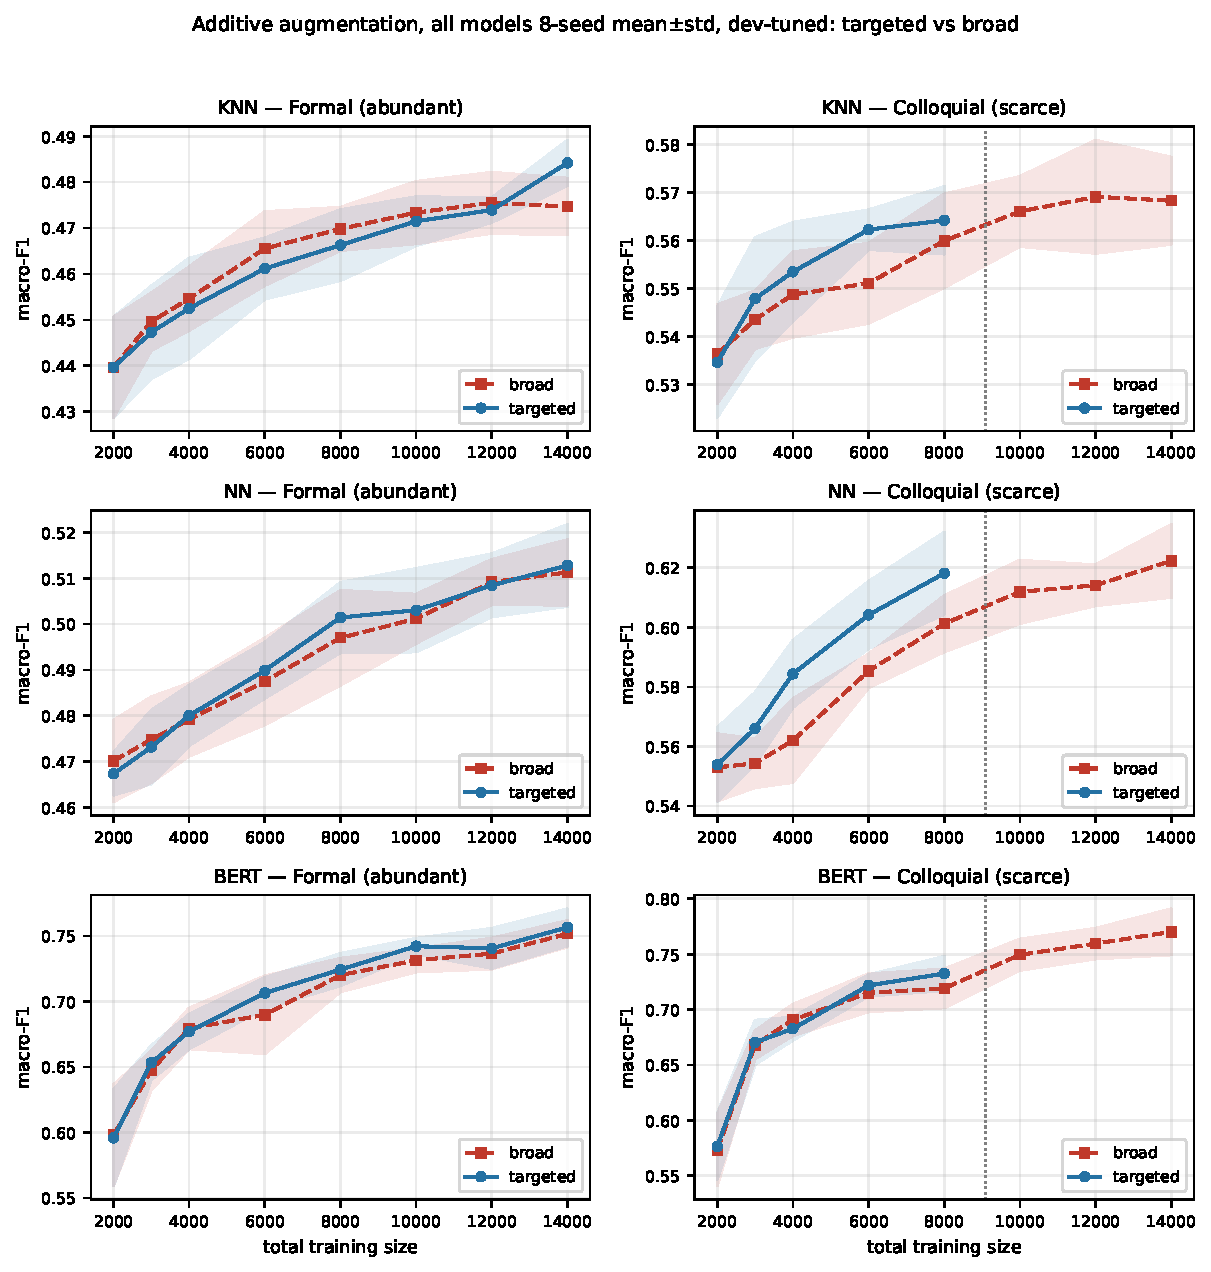
\includegraphics[width=\linewidth]{fig_augmentation.pdf}
\caption{$2{,}000$건 베이스라인에서의 가산 증강: targeted(in-domain) vs
broad(전체), KNN·NN·BERT(행). 각 곡선은 하이퍼파라미터 dev-선택 + 시드 $8$개
평균$\pm$표준편차, 증분 체크포인트. 같은 크기엔 targeted가 최소한 효율적이고, 표적
풀은 $9{,}000$ 부근서 고갈되며, 그 너머 broad 이득은 \emph{용량에 비례}한다---BERT는
$8$k$\to$$14$k서 $+0.037$ macro-F1, KNN·NN은 $\approx +0.004$.}
\label{fig:aug}
\end{figure}

발견 세 가지; 모두 arm당 시드 $8$개의 2-표본(Welch) $t$-검정으로 읽으며,
크기별 평균과 표준편차로부터 계산한다(유의 기준 $|t|>2.1$, $\alpha\approx.05$). \textbf{(i) 풍부한 도메인은 증강 구성이 무관.}
격식체에선 세 모델 모두 사실상 같은 수준이다---24개 (크기$\times$모델) 비교 중
22개가 비유의이고, 명목상 유의한 둘(KNN @$14{,}000$, $|t|=3.4$; BERT @$10{,}000$,
$|t|=2.8$)도 효과가 ${\le}0.011$ macro-F1, Bonferroni 미통과이며 일관된 방향이 없다
(KNN의 그 점은 다른 일곱 크기와 부호가 반대). $\alpha=.05$에서 24개 검정이면 우연히
${\approx}1.2$개가 유의해지므로, 격식체 결과는 무효과와 구분되지 않으며 구성 차이는
\emph{통계적 무}가 아니라 실무적으로 무시 가능으로 읽는다.
\textbf{(ii) 희소한 도메인은 같은 크기엔 in-domain이 더 효율적이나, 임베딩 기반
모델에 한해서다.} 구어체 $6{,}000$서 targeted가 broad를 유의하게 앞서는 건 NN
($+0.019$, $t=4.2$)과 KNN($+0.011$, $t=3.4$)뿐이고, BERT는 양의 차이지만 시드
노이즈 이내($+0.007$, $t=1.0$, 비유의)다. 이후 targeted는 $\approx 9{,}000$서 고갈.
\textbf{(iii) 그 너머 broad의 이득은 모델 용량에 비례한다.} 표적 천장($8{,}000$)$\to$broad
$14{,}000$은 동일하게 $6{,}000$건을 더하는 증분인데, 그 \emph{같은} 증분이 BERT는
$+0.037$($0.733\to0.770$, $t=4.1$) 올리지만 KNN·NN은 각 $+0.004$($|t|<1$)뿐이다.
각 모델의 천장까지 남은 헤드룸으로 정규화하면 격차는 더 뚜렷해진다---BERT는 그 거리의
약 $14\%$를 줄이는 반면 KNN·NN은 ${\approx}1\%$뿐이라, 절대 차이는 오히려 과소평가다.
증분이 모델 간 동일하므로 이는 데이터량 효과가 아니다: 자체 표현을 학습하는 모델은
추가 오프도메인에서 실제 신호를 뽑고, 고정 임베딩 모델은 거의 못 뽑는다. Bonferroni
보정(전 패밀리 ${\sim}40$개 targeted-vs-broad 검정, $\alpha\approx.0013$, $|t|>4.0$)에선
NN의 같은-크기 우위($t=4.2$)와 BERT의 용량 격차($t=4.1$)만 생존하고, KNN의 같은-크기
우위($t=3.4$)와 격식체의 두 고립점은 탈락한다. 유의 셀의 효과크기는 표준화 기준 크지만(Cohen's
$d\approx1.4$--$2.1$) 절대값으론 작다($1$--$2$ macro-F1점, 시드 분산이 작은 덕이다).
모든 모델이 동일하게 튜닝·평균(하이퍼파라미터 dev-선택: KNN $k$, NN 학습률
$\{0.003,\dots,0.1\}$ 발산 제외, BERT $3\times10^{-5}$; 각 곡선은 시드 $8$개 평균)되어
비교가 공정하다. 한 줄로: \emph{in-domain 증강은 저용량 모델에 한해 예제당 더
효율적이지만, 오프도메인으로 증강해야 할 때 계속 이득을 보는 건 고용량 모델뿐이다.}

\paragraph*{정확도를 넘어선 동작 읽기}
위 모든 곡선을 정확도가 아니라 매크로F1으로 읽는 이유는 둘이 모델별로 갈리기
때문이다. NumPy 신경망은 가장 쉬운 클래스를 과다 예측해 \emph{원시 정확도}를
끌어올릴 수 있는데, 이 붕괴는 세 클래스를 동등 가중하는 매크로F1이 벌점하지만
정확도는 가린다; 클래스별 정밀도·재현율을 매크로F1과 함께 추적해야 비로소 드러난다.
이는 발견이 아니라 \emph{보고 규율}이며, 위 비교들을 정확도로 읽지 않은 이유다.

%--------------------------------------------------------------
\section{한계}
\label{sec:limits}
첫째, 모든 수치는 KLUE-NLI와 고정된 범용 문장 임베딩 한정이다---시드 $8$개와
넓은 증강 크기를 스윕했으나 다중 데이터셋·인코더는 아니므로, 조건부 결론
(in-domain 증강이 과소대표 목표를 돕는다)은 외부 재현이 필요하다. 효과 크기도
작고($1$--$2$ macro-F1점) 임베딩 기반 두 모델(KNN·NN)에서 뚜렷하며, 각 모델은 dev로 튜닝돼 곡선이
망가진 게 아니라 튜닝된 학습기를 반영한다. 둘째, 전제와 가설을 한 벡터 $\phi$로 합치면 BERT 같은 조인트 어텐션이
잡는 토큰 상호작용 일부를 잃는다---임베딩 기반 분류기의 구조적 불리이며, 튜닝으로
없앨 결함이 아니다. 셋째, LSP/OCP 증거는 설계 수준(같은 호출 지점, 서브클래스
추가)이지 정량적 유지보수성 측정은 범위 밖이다. 각 한계의 개선: $\phi$를
크로스-인코더 \texttt{Embedder}로 대체(분류기 불변, OCP); 시드·데이터셋 확장; 새
모델 추가 시 바뀐 코드 줄 수로 OCP를 정량화.

%--------------------------------------------------------------
\section{결론}
\label{sec:conclusion}
세 분류기를 하나의 \texttt{Classifier} 추상 아래, 두 데이터 전략을
\texttt{Domain}/\texttt{TrainingStrategy} 아래 두고 한국어 NLI에서 비교했다. 작은
in-domain 베이스라인을 증강하며 각 목표의 test 슬라이스로 평가한 결과, 풍부한
목표에선 증강 구성이 실무적으로 무차이였고(명목상 유의한 소수 점은 노이즈 수준·
보정 미통과), 희소 목표에선 같은 크기의 in-domain(targeted) 우위가 작고 저용량
모델(NN·KNN, BERT 아님)에 한정되며 그나마 희소 풀에 막혔다. 가장 분명한---그리고
다중비교 보정 후 유일하게 살아남는---효과는 그 천장 너머에 있었다: broad(오프도메인)
증강의 한계 이득이 모델 용량에 비례해, 고용량 BERT만 $+0.037$ macro-F1(남은 헤드룸의
약 $14\%$)을 얻고 KNN·NN은 $\approx +0.004$에 그쳤다. 정확도가 아니라
매크로F1과 혼동행렬을 보고한 것이 이를 드러내는 데 필수였다.

더 넓은 동기는 데이터 \emph{적합성}이다. 유비로서---오직 유비로서---이는 생성형
멀티에이전트 시스템을 닮았다: 각 이질적 에이전트의 약점에 표적화된 데이터로
증강할까, 공유 풀을 증강할까? 우리 결과는 소외된(과소대표) 대상일수록 표적
증강이 값어치를 하지만 그 데이터는 양이 제한적이고 공유 풀 증강은 그 대상엔 일찍
포화함을 시사한다(분류기는 그런 에이전트의 proxy일 뿐, 유비이지 동일성 아님).
유일한 구체 기술 연결은 BERT 계열 문장 임베딩이 우리 특징 공간과 현대 의미
매칭의 근간이라는 점이다. 더 많은 시드·실제 합성 증강·진짜 에이전트별 약점으로의
확장은 향후 과제로 남긴다.

\paragraph*{배운 점}
세 가지 객체지향 교훈을 얻었다. 첫째, 추상화가 제값을 했다---\texttt{Classifier}를
한 번 정의하니 매우 다른 세 모델이 같은 평가 코드를 공유했고, 실험이 구동부
재작성 대신 서브클래스 추가로 자랐다. 둘째, 추상의 \emph{경계}가 교훈적이었다---
KNN/NN은 \texttt{Embedder} 출력을, BERT는 원시 텍스트를 소비하며, 공유 인터페이스가
\emph{호출 지점}을 통일하되 표현은 각자 필요한 것을 있는 그대로 받게 두는 것이
억지 통일보다 나은 설계였다. 셋째, 작은 규율이 실전에서 중요했다---
\texttt{from\_dict} 팩토리와 커스텀 \texttt{InvalidSampleError}가 잘못된 행을 모델
이전에 걸러냈고, 역전파를 직접 구현한 덕에 신경망이 블랙박스에서 추론·디버깅
가능한 것으로 바뀌었다.

%--------------------------------------------------------------
\bibliographystyle{IEEEtran}
\bibliography{refs}

\end{document}
